\documentclass[12pt]{article}
\usepackage{graphicx} % Required for inserting images
\usepackage[dvipsname]{xcolor}
\usepackage[margin=1in]{geometry}
\usepackage{amsmath}
\usepackage{tikz, tcolorbox}
\usepackage{hyperref}
\usepackage{setspace}
\doublespacing


\begin{document}
\setlength{\parindent}{1mm}
\setlength{\parskip}{1mm}

\begin{center}
\textbf{\LARGE Prey-Predator Dynamics Simulation}\\[10pt]
\textbf{Abhishek Biswas$^1$}\\
Email: abhishekbiswas2006@gmail.com\\[15pt]

\textit{This report has been uploaded to \href{https://github.com/Abhishek9824/prey-predator-dynamics-simulation}{\textbf{}GitHub} for public access. }

{\color{blue}Published Date: 27 July, 2025}
\end{center}



\rule{\textwidth}{0.5pt}

\section{Introduction}
After Alan Turing expressed, "the world is a differential equation" which is true. We can abtract equation mathematically or model nature phenonemon mathematically which can analyze further and propose theory and equation. Mathematically model is one among the good tools that enable to model and analyze complex real-world systems through mathematical equations, resulting in insights, prediction, and optimized solutions.
\section{Prey-Predator Model}
The prey-predator model describes the relationship between two groups of animals in nature one prey and another predator. Once predators become plentiful, they eat more prey, causing the prey population to drop. With less food available, some predators can’t survive or have fewer babies, so their numbers shrink. This allows the prey to increase again, and the cycle continues in a repeating pattern. This model shows how the populations of prey and predators are closely linked and constantly affect each other, highlighting the balance and connectedness of nature.\\
The Lotka-Volterra model is a foundational mathematical framework used to describe how the populations of two interacting species—typically one prey and one predator—change over time. Developed independently by Alfred Lotka and Vito Volterra in the 1920s, these Lotka-Volterra equations are a set of first-order, nonlinear differential equations that model the cyclical dynamics often observed in natural predator-prey systems.
\begin{align}
    \frac{dx}{dt}=\alpha x-\beta x y
\end{align}
\begin{align}
    \frac{dy}{dt}=\delta xy-\gamma y 
\end{align}\\
Where,
\begin{align}
$x$= size of the prey population (e.g., Deers)

$y$= size of the predator population (e.g., Wolves)

$\alpha$ = natural growth rate of the prey in the absence of predators

$\beta$ = rate at which predators kill prey

$\gamma$ = natural death rate of the predators in the absence of food

$\delta$ = rate at which predators increase by consuming prey
\end{align}
\section{Method}
\begin{tcolorbox}[title=Defining Time]
    t = np.linspace(0, 50, num=1000)
\end{tcolorbox}
t= time, this helps to creates a timeline from 0 to 50 (days/months) and 
1000 points how smooth and detailed it will be.\\

Next, Setting up the parameters:
\begin{tcolorbox}[title= Model Parameters]
alpha = 1.1   # growth rate of deer\\
beta = 0.4    # rate wolves eat deer\\
delta = 0.1   # rate wolves increase from eating deer\\
gamma = 0.4   # death rate of wolves
\end{tcolorbox}
\textbf{Special case:} Steady-state conditon is refers to as rate of input and output variables are balanced or no net change in the ecosystem.

\begin{tcolorbox}[title= Steady-State Condition]
    y0 = [gamma/delta , alpha/beta]
\end{tcolorbox}

\begin{tcolorbox}[title= Model Function] 
    def sim(variables, t, params):\\
    x = variables[0]  # prey (deer)\\
    y = variables[1]  # predator (wolves)\\

    alpha = params[0]\\
    beta = params[1]\\
    delta = params[2]\\
    gamma = params[3]\\

    dxdt = alpha*x - beta*x*y \\ 
    dydt = delta*x*y - gamma*y\\

    return [dxdt, dydt]

\end{tcolorbox}

\subsection{Result and Analysis}
The simulated dynamics of wolves and deer are classic predator–prey cycles. Deer increase first as a function of vegetation availability, then experience a time-lagged increase in wolves as a consequence of ample prey. Enhanced predation brings deer numbers down, followed by a subsequent decline in wolves. This establishes a repeating cycle with a distinct time lag between species peaks. The phase plot is a closed loop, demonstrating the stable, oscillatory relationship between predator and prey.
\begin{figure}[h]
    \centering
    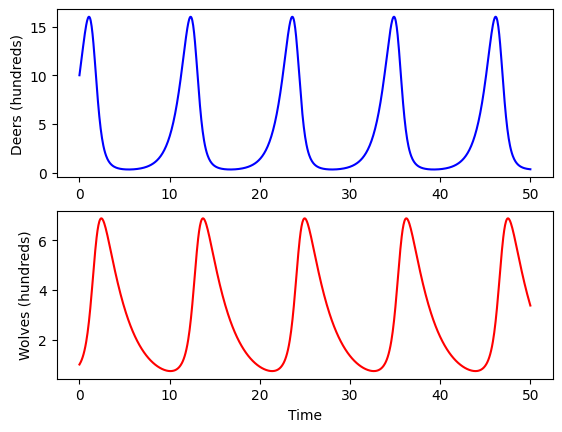
\includegraphics[scale=1]{Dynamics.png}
    \caption{Result of two-species interaction}
    \label{fig:enter-label}
\end{figure}
\subsection{Phase Space Plot}
A phase space plot is a type of graph that shows how two variables (often from a dynamical system) relate to each other but not over time, but with respect to each other. \\
The phase plot of prey versus predators displays a closed-loop trajectory, indicating stable, cyclic population dynamics. As the prey population rises, predator numbers follow with a time delay, eventually causing a decline in prey due to predation. This leads to a subsequent decline in predators, after which the prey population recovers. The repeating loop in phase space illustrates the classic predator–prey feedback cycle and confirms the presence of stable oscillations in the system.



\begin{figure}[h]
    \centering
    \includegraphics[scale=0.8]{download.png}
    \caption{Phase-Space plot: predators vs prey}
    \label{fig:enter-label}
\end{figure}

\section{Three Species in Ecological Modeling}
In traditional ecological models like the Lotka–Volterra predator–prey model, interactions are simulated between only two species: usually one predator and one prey. Useful as these two-species models are, they are simplifications and do not always represent the richness of real ecosystems, in which species are part of multi-trophic food webs or chains.
\newpage

Deriving the equation for three species interactions,\\[10pt]
for Grass Population(G),
$$\frac{dG}{dt}=rG(1-\frac{G}{K})-aGD$$

for Deer Population(D),
$$\frac{dD}{dt}=bGD-cDW-dD$$

for Wolves Population(W),
$$\frac{dW}{dt}=eDW-fW$$

where,
\begin{align}

$r$ = Grass growth rate

$K$ = Grass carrying capacity

$a$ = Grass consumption rate by deer

$b$ = Conversion rate of plants to deer biomass

$c$ = predation rate of wolves

$d$ = natural death rate of deer

$e$ = Efficiency of converting prey to predator

$f$ = Death rate of wolves
\end{align}

\subsection{Result and Analysis}
The population vs. time plot shows a characteristic trophic cascade behavior in the three-species model. Initially, the plant population increases rapidly due to low herbivore pressure. This is followed by multiple oscillations in the herbivore (deer) and predator (wolf) populations, with predator peaks lagging slightly behind prey peaks—consistent with classical predator–prey dynamics.
However, the oscillations are damped over time, and the system reaches a stable equilibrium. The final population levels suggest a top-down controlled system: wolves maintain a high population, deer are suppressed to near-extinction levels, and plant biomass stabilizes due to low grazing pressure. This reflects a realistic ecological scenario in which a dominant predator indirectly facilitates plant persistence by controlling herbivore abundance.

\begin{figure}
    \centering
    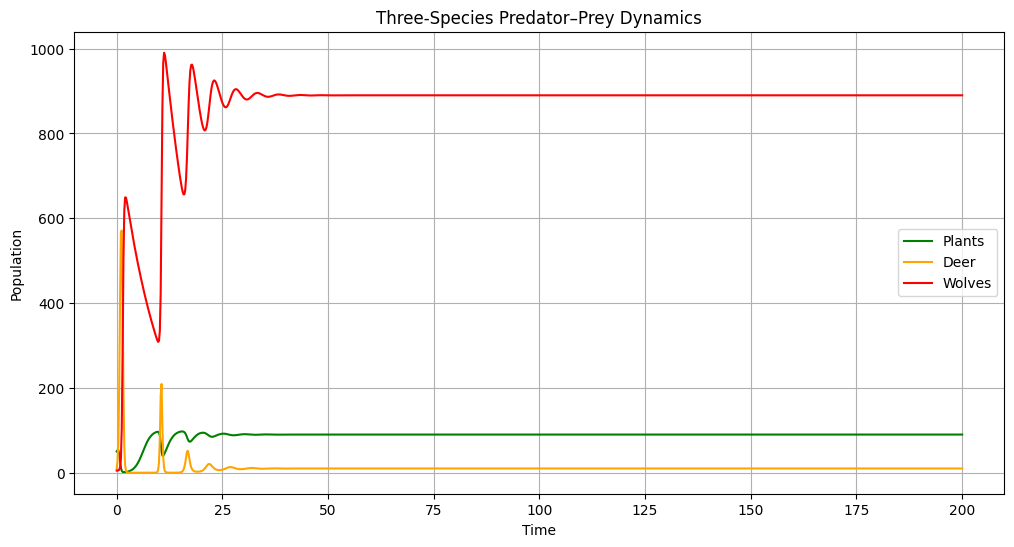
\includegraphics[scale=0.6]{Three Speciee PPD.png}
    \caption{Result of three-species interaction}
    \label{fig:enter-label}
\end{figure}


























\end{document}